\documentclass{article}

% Language setting
% Replace `english' with e.g. `spanish' to change the document language
\usepackage[english]{babel}

% Set page size and margins
% Replace `letterpaper' with `a4paper' for UK/EU standard size
\usepackage[letterpaper,top=2cm,bottom=2cm,left=3cm,right=3cm,marginparwidth=1.75cm]{geometry}

% Useful packages
\usepackage{amsmath}
\usepackage{amssymb}
\usepackage{amsfonts}
\usepackage{cancel}
\usepackage{graphicx}
\usepackage[colorlinks=true, allcolors=blue]{hyperref}

\usepackage{natbib}

\title{Evolutionary Transducer}
\author{Ian Holmes}

\begin{document}
%\maketitle

\section{Statistical alignment}

\subsection{Transducer composition}

\newcommand\gappedalphabet{(\Omega \cup \{\epsilon\})}

For our purposes, a transducer is a tuple
$\mathbb{T} = (\Omega, \Phi, \phi_0, \Psi, \tau)$
where
$\Omega$ is an alphabet,
$\Phi$ is a set of states,
$\phi_0 \in \Phi$ is the start state,
$\Psi \subseteq \Phi$ are the end states, 
$\tau:\mathfrak{T} \to \Re$ is the transition weight function,
$\mathfrak{T} = \Phi \times \gappedalphabet \times \gappedalphabet \times \Phi$ is the labeled transition relation,
and $\epsilon$ is the empty string.

A transition $(i,x,y,j) \in \mathfrak{T}$ has source and destination states $i,j$ and input and output labels $x,y$.
For input and output sequences ${\cal X}, {\cal Y} \in \Omega^\ast$
define the Forward\footnote{So-called because it can be computed by the Forward algorithm, after marginalizing any null transition cycles.} weight
$\mathbb{T}_{\cal XY}$ to be the sum of weights of all paths from $\phi_0$ to any $\psi \in \Psi$
such that the concatenated input and output labels are, respectively, ${\cal X}$ and ${\cal Y}$, where the weight of a path is defined as the product of its transition weights.
Two transducers are considered equivalent if their Forward weights are equal for all input and output sequences.

A transition is an ``input'' if its input label is not $\epsilon$, and ``null'' if both its input and output labels are $\epsilon$.
The ``outgoing transitions'' of a state are all the finite-weight transitions whose source is that state.
A state ``waits'' if all its outgoing transitions (if there are any) are inputs,
and ``continues'' if (i) it has at least one outgoing transition and (ii) none of its outgoing transitions are inputs.
A transducer is a ``waiting machine'' if all its states either wait or continue.
Any transducer can be transformed into an equivalent waiting machine by adding an extra state and null transition to split any state
that doesn't meet the requirement.

A composition of two transducers $\mathbb{A},\mathbb{B}$ is a transducer $\mathbb{AB}$ representing the matrix product
\[
(\mathbb{AB})_{{\cal XZ}} = \sum_{{\cal Y} \in \Omega^\ast} \mathbb{A}_{\cal XY} \mathbb{B}_{\cal YZ} \ \forall\ {\cal X},{\cal Z} \in \Omega^\ast
\]
To establish the existence of at least one such transducer it's sufficient to consider the case where $\mathbb{B}$ is a waiting machine.
Take the Cartesian product of $\mathbb{A}$'s and $\mathbb{B}$'s state spaces and synchronize transitions,
so that $\mathbb{A}$'s output labels match $\mathbb{B}$'s input labels and $\mathbb{B}$ must be in a wait state before $\mathbb{A}$ can transition
\[
  \tau_{\mathbb{AB}}((i,i'),x,z,(j,j')) = \left\{
  \begin{array}{ll}
    \tau_{\mathbb{A}}(i,x,\epsilon,j) + \displaystyle \sum_{y \in \Omega} \tau_{\mathbb{A}}(i,x,y,j) \tau_{\mathbb{B}}(i',y,\epsilon,i') & \mbox{if $i'$ waits, $j' = i'$, and $z = \epsilon$} \\
    \displaystyle \sum_{y \in \Omega} \tau_{\mathbb{A}}(i,x,y,j) \tau_{\mathbb{B}}(i',y,z,j') & \mbox{if $i'$ waits and $j' \neq i'$} \\
    \tau_{\mathbb{B}}(i',\epsilon,z,j') & \mbox{if $i'$ continues, $j = i$, and $x = \epsilon$} \\
    0 & \mbox{otherwise}
  \end{array} \right.
\]
Note this composition preserves alignment transitivity: characters that are aligned\footnote{In the sense of being associated with the same transition, on a given state path.}
through both $\mathbb{A}$ and $\mathbb{B}$ are aligned by $\mathbb{AB}$ with the same weight.
We will require this to be true of all transducer compositions we consider:
it's how we map transitions from composite machines to simpler machines.

\subsection{State-based emissions}

A transducer has state-based emissions if its state space can be partitioned into
match, insert, delete, and null states $\{ \sigma_M, \sigma_I, \sigma_D, \sigma_N \}$
such that for all transitions $(i,x,y,j)$ of finite weight, exactly one of the following is true
\begin{eqnarray*}
  j \in \sigma_M: & x \in \Omega, & y \in \Omega \\
  j \in \sigma_I: & x = \epsilon, & y \in \Omega \\
  j \in \sigma_D: & x \in \Omega, & y = \epsilon \\
  j \in \sigma_N: & x = \epsilon, & y = \epsilon
\end{eqnarray*}
and further $\tau(i,x,y,j) = U_{ij} E_j(x,y)$ where ${\bf U}$ is a transition matrix and $E_j$ an emission weight.

Any transducer can be transformed into an equivalent state-based emitter by adding states.

\subsection{Expected transition count $T_{XY}$}

Given a conditionally-normalized\footnote{Meaning the Forward weight is a probability whose sum over output sequences, for any given input sequence, is 1.}
state-based emitter with exactly one match state $\sigma_M = \{ 1 \}$,
we seek $T_{XY}$, the expected number of times that the shortest closed walk from/to state 1,
with its null states removed, includes a transition from $\sigma_X$ to $\sigma_Y$.

\newcommand\nottomatch{L}
\newcommand\notfrommatch{R}
\newcommand\tox{X}
\newcommand\tonull{N}
\newcommand\xtoy{{X \to Y}}

Define some indicator matrices
${\bf J}^\xtoy$,
${\bf J}^\tox$
(for $X,Y \in \{ M, I, D, N \}$) and
${\bf J}^\nottomatch$,
${\bf J}^\notfrommatch$

\begin{eqnarray*}
  J^\xtoy_{ij} & = & \left\{ \begin{array}{ll} 1 & \mbox{if $i \in \sigma_X$ and $j \in \sigma_Y$} \\ 0 & \mbox{if $i \notin \sigma_X$ or $j \notin \sigma_Y$} \end{array} \right. \\
  J^\tox_{ij} & = & \left\{ \begin{array}{ll} 1 & \mbox{if $j \in \sigma_X$} \\ 0 & \mbox{if $j \notin \sigma_X$} \end{array} \right. \\
  J^\nottomatch_{ij} & = & \left\{ \begin{array}{ll} 1 & \mbox{if $j \notin \sigma_M$} \\ 0 & \mbox{if $j \in \sigma_M$} \end{array} \right. \\
  J^\notfrommatch_{ij} & = & \left\{ \begin{array}{ll} 1 & \mbox{if $i \notin \sigma_M$} \\ 0 & \mbox{if $i \in \sigma_M$} \end{array} \right.
\end{eqnarray*}

Let ${\bf U}$ be the transition matrix.
Then

\begin{eqnarray*}
T_{XY} & = &
\left(
\left( {\bf I} - {\bf J}^\nottomatch \odot {\bf U} \right)^{-1}
\left(
     {\bf J}^\xtoy \odot
     \left(
     \left( {\bf I} - {\bf J}^\tonull \odot {\bf U} \right)^{-1}
          {\bf U}
     \right)
\right)
\left( {\bf I} - {\bf J}^\notfrommatch \odot {\bf U} \right)^{-1}
\right)_{11}
\end{eqnarray*}

Here $\odot$ is the elementwise product.



\subsection{Rate of change $R_{XY}$ of expected transition count}

Suppose that
$\mathbb{Q}$ is the generator for an indel process,
$\mathbb{G}(\delta_t) = \mathbb{I} + \mathbb{Q} \delta_t$ is the infinitesimal transducer,
$\mathbb{F}(t)$ the finite-time approximator\footnote{Alternatively, $\mathbb{F}$ can be an HMM whose output approximates the equilibrium distribution of $\mathbb{Q}$ as $t \to \infty$.},
and $\mathbb{FG}$ the transitively-aligning composition of $\mathbb{F}$ and $\mathbb{G}$.

Let ${\bf U}(\theta,t,\delta_t)$ be the transition matrix
of the composite machine $\mathbb{FG}$
at time $t$, infinitesimal time increment $\delta_t$, and parameter value $\theta$.
By the definition of $\mathbb{G}$ this is first-order in $\delta_t$, so it has the form
\[
  {\bf U}(\theta,t,\delta_t) = {\bf U}_0(\theta,t) + {\bf U}_t(\theta,t) \delta_t
  \]

We are interested in
\begin{eqnarray*}
\frac{\partial}{\partial t}T_{XY} & = & \lim_{\delta_t \to 0} \frac{T_{XY}(\theta,t,\delta_t) - T_{XY}(\theta,t,0)}{\delta_t} \\
\frac{\partial^2}{\partial \theta \partial t}T_{XY} & = & \lim_{\delta_\theta \to 0} \lim_{\delta_t \to 0}
\frac{\left(T_{XY}(\theta+\delta_\theta,t,\delta_t) - T_{XY}(\theta+\delta_\theta,t,0)\right) - \left(T_{XY}(\theta,t,\delta_t) - T_{XY}(\theta,t,0)\right)}{\delta_\theta \delta_t}
\end{eqnarray*}
We will use the time derivative to numerically integrate $T_{XY}$, and the cross partial derivative for parameter-fitting.
For later convenience define $R_{XY} \equiv \frac{\partial}{\partial t} T_{XY}$.

Expand ${\bf U}$ to first order in both $\delta_\theta$ and $\delta_t$
\newcommand\tthetaexpansion[2]{  {#2}_0^{#1}
  + {#2}_\theta^{#1} \delta_\theta
  + {#2}_t^{#1} \delta_t
  + {#2}_{\theta t}^{#1} \delta_\theta \delta_t }
\newcommand\uexpansion{\tthetaexpansion{}{\bf U}}
\newcommand\vexpansion[1]{\tthetaexpansion{#1}{\bf V}}
\[
  {\bf U}(\theta+\delta_\theta,t,\delta_t) = \uexpansion + O(\delta_\theta^2) % + O(\delta_t^2)
\]
where ${\bf U}_0={\bf U}(\theta,t,0)$,
${\bf U}_t=\frac{1}{\delta_t} \left( {\bf U}(\theta,t,\delta_t) - {\bf U}(\theta,t,0) \right)$,
${\bf U}_\theta=\frac{\partial}{\partial \theta} {\bf U}_0$,
${\bf U}_{\theta t}=\frac{\partial}{\partial \theta}  {\bf U}_t$.

We can now expand the matrix inverses.
In general, for $x \in \{ \nottomatch, \tonull, \notfrommatch \}$,
\begin{eqnarray*}
  \left( {\bf I} - {\bf J}^x \odot {\bf U} \right)^{-1}
%  & = &
%  \left( {\bf I} - {\bf J}^x \odot {\bf U}_0
%  - {\bf J}^x \odot {\bf U}_\theta \delta_\theta
%  - {\bf J}^x \odot {\bf U}_t \delta_t
%  - {\bf J}^x \odot {\bf U}_{\theta t} \delta_\theta \delta_t
%  + O(\delta_\theta^2) + O(\delta_t^2)
%  \right)^{-1} \\
%  & = &
%  \left(
%  \left( {\bf I} - {\bf J}^x \odot {\bf U}_0 \right)
%  \left( {\bf I}
%  - {\bf V}^x_0 \left( {\bf J}^x \odot {\bf U}_\theta \delta_\theta
%  + {\bf J}^x \odot {\bf U}_t \delta_t
%  + {\bf J}^x \odot {\bf U}_{\theta t} \delta_\theta \delta_t
%  \right) \right)
%  + O(\delta_\theta^2) + O(\delta_t^2)
%  \right)^{-1} \\
%  & = &
%  \left(
%  \left( {\bf I}
%  + {\bf V}^x_0 \left( {\bf J}^x \odot {\bf U}_\theta \delta_\theta
%  + {\bf J}^x \odot {\bf U}_t \delta_t
%  + {\bf J}^x \odot {\bf U}_{\theta t} \delta_\theta \delta_t
%  \right)
%  \right) \right)
%  {\bf V}^x_0
%  + O(\delta_\theta^2) + O(\delta_t^2) \\
%  & = &
%  {\bf V}^x_0
%  + {\bf V}^x_0 \left( {\bf J}^x \odot {\bf U}_\theta \right) {\bf V}^x_0 \delta_\theta
%  + {\bf V}^x_0 \left( {\bf J}^x \odot {\bf U}_t \right) {\bf V}^x_0 \delta_t
%  + {\bf V}^x_0 \left( {\bf J}^x \odot {\bf U}_{\theta t} \right) {\bf V}^x_0 \delta_\theta \delta_t
%  + O(\delta_\theta^2) + O(\delta_t^2) \\
  & = & \vexpansion{x} + O(\delta_\theta^2) + O(\delta_t^2) \\
{\bf V}^x_0 & = & ({\bf I} - {\bf J}^x \odot {\bf U}_0)^{-1} \\
{\bf V}^x_\theta & = & {\bf V}^x_0 \left( {\bf J}^x \odot {\bf U}_\theta \right) {\bf V}^x_0 \\
{\bf V}^x_t & = & {\bf V}^x_0 \left( {\bf J}^x \odot {\bf U}_t \right) {\bf V}^x_0 \\
{\bf V}^x_{\theta t} & = & {\bf V}^x_0 \left( {\bf J}^x \odot {\bf U}_{\theta t} \right) {\bf V}^x_0
\end{eqnarray*}

Thus
\begin{eqnarray*}
T_{XY} & = &
\left(
\left( \vexpansion\nottomatch \right)
\right. \\ & & \quad \times
\left(
     {\bf J}^\xtoy \odot
     \left( \left( \vexpansion\tonull \right)
     \left( \uexpansion \right) \right)
\right)
 \\ & & \quad \left. \times
 \left( \vexpansion\notfrommatch \right)
\right)_{11}  + O(\delta_\theta^2) + O(\delta_t^2)
\end{eqnarray*}

For convenience define
\begin{eqnarray*}
W_{a,b,c,d} & = &
\left( {\bf V}^\nottomatch_a \left( {\bf J}^\xtoy \odot \left( {\bf V}^\tonull_b {\bf U}_c \right) \right) {\bf V}^\notfrommatch_d \right)_{11}
\end{eqnarray*}
Examining the coefficients of $\delta_t$ and $\delta_\theta \delta_t$, we see that

\begin{eqnarray*}
  R_{XY} & = &
  W_{t,0,0,0} + W_{0,t,0,0} + W_{0,0,t,0} + W_{0,0,0,t}
  \\
  \frac{\partial}{\partial \theta}R_{XY} & = &
  W_{t,\theta,0,0} + W_{t,0,\theta,0} + W_{t,0,0,\theta}
  + W_{\theta,t,0,0} + W_{0,t,\theta,0} + W_{0,t,0,\theta}
  + W_{\theta,0,t,0} + W_{0,\theta,t,0} + W_{0,0,t,\theta}
  \\ & &
  + W_{\theta,0,0,t} + W_{0,\theta,0,t} + W_{0,0,\theta,t}
  + W_{\theta t,0,0,0} + W_{0,\theta t,0,0} + W_{0,0,\theta t,0} + W_{0,0,0,\theta t}
\end{eqnarray*}

This first-order expansion allows us to ``differentiate through'' the matrix inverse.
%These equations remain valid if the parameter $\theta$, with respect to which we are differentiating, is itself one of the $T_{XY}$
%(since these are parameters of $\mathbb{F}$ and hence of ${\bf U}$).

\subsection{Expected state count $S_X$}

In order to parameterize $\mathbb{F}$ using $\{ T_{XY} \}$, we need to normalize by $S_X$, the expected number of $\sigma_X$-states entered by the walk.
Note that $S_x = \sum_{y \in \{M,I,D\}} T_{xy}  = \sum_{y \in \{M,I,D\}} T_{yx}$
and $S_M = 1$.
Thus if we have all the $\{ T_{XY} \}$ then we can trivially find the $\{ S_X \}$.

Sometimes it may be useful to compute the $S_X$ separately:

\begin{eqnarray*}
S_X & = &
\left(
     \left(
          {\bf J}^\tox \odot
          \left( {\bf I} - {\bf J}^\nottomatch \odot {\bf U} \right)^{-1}
     \right)
\left( {\bf I} - {\bf J}^\notfrommatch \odot {\bf U} \right)^{-1}
\right)_{11}
\\
& = &
\left(
     \left(
          {\bf J}^\tox \odot
          \left( \vexpansion\nottomatch \right)
     \right)
\left( \vexpansion\notfrommatch \right)
\right)_{11}  + O(\delta_\theta^2) + O(\delta_t^2)
  \\
\frac{\partial}{\partial t} S_X & = &
  W'_{t,0} + W'_{0,t}
  \\
\frac{\partial^2}{\partial \theta \partial t} S_X & = &
  W'_{t,\theta} + W'_{\theta,t}
  + W'_{\theta t,0} + W'_{0,\theta t}
\\
W'_{a,b} & = &
\left( \left( {\bf J}^\tox \odot {\bf V}^\nottomatch_a \right) {\bf V}^\notfrommatch_b \right)_{11}
\end{eqnarray*}

The approach in \cite{Holmes2020} (following \cite{DeMaio2020}) is to find $S_X$ for the transition matrix of $\mathbb{F}$ using
the first of the above equations, then to express $\frac{\partial}{\partial t} S_X = \sum_y R_{YX}$
in terms of this, obtaining a solvable ODE for $S_X$.


\subsection{Runge-Kutta recursions for $T_{XY}$ and derivatives}

Let ${\bf R} \equiv {\bf R}(\Theta,{\bf T})$,
where $\mathbb{G} \equiv \mathbb{G}(\Theta,\delta_t)$
and $\mathbb{F} \equiv \mathbb{F}({\bf T},t)$.

${\bf R}$ includes all the $R_{XY}$, as ${\bf T}$ includes the $T_{XY}$, and $\Theta$ the infinitesimal model parameters.

We use the Runge-Kutta method (RK4) to numerically integrate $\dot{\bf T}={\bf R}$
so as to estimate $T_{XY}(t)$ at timepoints $(t_0=0, t_1, t_2 \ldots)$.
Let $\Delta_n = t_{n+1}-t_n$.
Applying RK4 gives

\begin{eqnarray*}
  {\bf T}^{(n+1)} & = & {\bf T}^{(n)} + \frac{\Delta_n}{6} \left( {\bf K}^{(n,1)} + 2{\bf K}^{(n,2)} + 2{\bf K}^{(n,3)} + {\bf K}^{(n,4)} \right) \\
  {\bf K}^{(n,1)} & = & {\bf R}\left(\Theta,{\bf T}^{(n)}\right) \\
  {\bf K}^{(n,2)} & = & {\bf R}\left(\Theta,{\bf T}^{(n)} + \frac{\Delta_n}{2} {\bf K}^{(n,1)}\right) \\
  {\bf K}^{(n,3)} & = & {\bf R}\left(\Theta,{\bf T}^{(n)} + \frac{\Delta_n}{2} {\bf K}^{(n,2)}\right) \\
  {\bf K}^{(n,4)} & = & {\bf R}\left(\Theta,{\bf T}^{(n)} + \Delta_n {\bf K}^{(n,3)}\right)
\end{eqnarray*}

For any parameter $\theta \in \Theta$ we can use the chain rule to find the derivative

\newcommand\ptheta{\frac{\partial}{\partial\theta}}
\newcommand\ptxy{\frac{\partial}{\partial T_{XY}}}
\newcommand\allpartials[1]{\ptheta #1 + \sum_{X,Y} \ptxy #1 \ptheta T_{XY}^{(n)}}
\newcommand\allpartialsk[3]{\ptheta #1 + \sum_{X,Y} \ptxy #1 \left( \ptheta T_{XY}^{(n)} + #2 \ptheta K_{XY}^{(n,#3)} \right)}
\begin{eqnarray*}
  \ptheta {\bf T}^{(n+1)} & = & \ptheta {\bf T}^{(n)} + \frac{\Delta_n}{6} \left( \ptheta {\bf K}^{(n,1)} + 2\ptheta{\bf K}^{(n,2)} + 2\ptheta{\bf K}^{(n,3)} + \ptheta{\bf K}^{(n,4)} \right) \\
  \ptheta {\bf K}^{(n,1)} & = & \allpartials{{\bf R}\left(\Theta,{\bf T}^{(n)}\right)} \\
  \ptheta {\bf K}^{(n,2)} & = & \allpartialsk{{\bf R}\left(\Theta,{\bf T}^{(n)} + \frac{\Delta_n}{2} {\bf K}^{(n,1)}\right)}{\frac{\Delta_n}{2}}{1} \\
  \ptheta {\bf K}^{(n,3)} & = & \allpartialsk{{\bf R}\left(\Theta,{\bf T}^{(n)} + \frac{\Delta_n}{2} {\bf K}^{(n,2)}\right)}{\frac{\Delta_n}{2}}{2} \\
  \ptheta {\bf K}^{(n,4)} & = & \allpartialsk{{\bf R}\left(\Theta,{\bf T}^{(n)} + \Delta_n {\bf K}^{(n,3)}\right)}{\Delta_n}{3}
\end{eqnarray*}

\subsection{Infinitesimal transducer $\mathbb{G}$ for General Geometric Indel model (GGI)}

A sequence ${\cal S}(t)$ evolves by
substitutions (rate matrix ${\bf Q}$),
deletions (rate $\mu$ per site, extension probability $y$),
and
insertions (rate $\lambda$, extension $x$,
characters $\sim {\bf Q}$'s stationary distribution $\pi$).

At equilibrium, sequence length $\sim$ Geometric($\lambda/\mu$). Character frequencies $\pi$.

If the model is required to be reversible then $\lambda y(1-x) = \mu x(1-y)$.

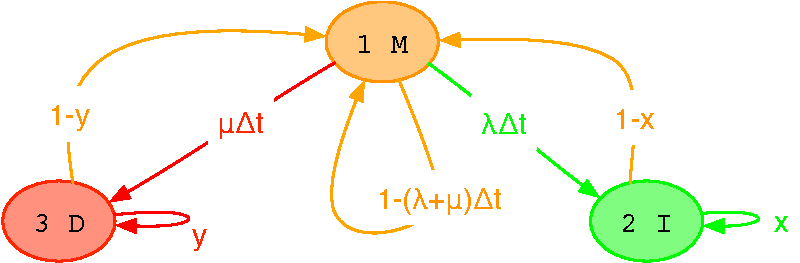
\includegraphics[width=\textwidth]{InstantHMM.pdf}

To calculate gap length distributions inside the sequence, it's convenient to ignore end effects,
assuming instead that the sequence is infinitely long.
We can then dispense with start and end states, as shown in the figure on the left.
(For finite-length sequences, we could use the version on the right.)

\subsection{Approximate finite-time transducer $\mathbb{F}$ for GGI model}

A transducer whose Forward likelihood approximates $P({\cal S}(t)|{\cal S}(0))$

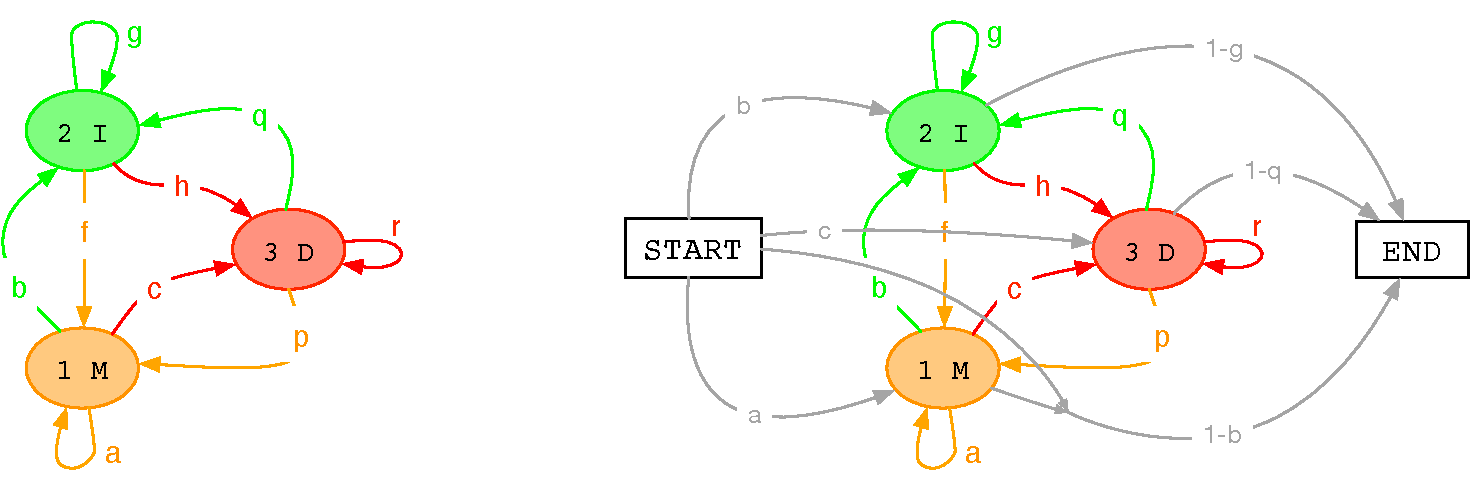
\includegraphics[width=\textwidth]{PairHMM.pdf}

Again, the version on the left is for infinite sequences; on the right, finite sequences.

At $t=0$: $a(0)=1$, $f(0)=1-x$, $g(0)=x$, $p(0)=1-y$, $r(0)=y$, and $b(0)=c(0)=h(0)=q(0)=0$.

For $t>0$, % following Holmes (2020)
\begin{eqnarray*}
\begin{pmatrix}
a & b & c \\
f & g & h \\
p & q & r 
\end{pmatrix}
& = &
\begin{pmatrix}
T_{MM} / S_M & T_{MI} / S_M & T_{MD} / S_M \\
T_{IM} / S_I & T_{II} / S_I & T_{ID} / S_I \\
T_{DM} / S_D & T_{DI} / S_D & T_{DD} / S_D 
\end{pmatrix}
\\
& = &
\begin{pmatrix}
T_{MM} & T_{MI} & 1-T_{MM}-T_{MI} \\
T_{IM}/S_I & (S_I-T_{MI}-T_{DI})/S_I & (T_{MI}+T_{DI}-T_{IM})/S_I \\
(1-T_{MM}-T_{IM})/S_D & T_{DI}/S_D & (S_D+T_{MM}+T_{IM}-T_{DI}-1)/S_D 
\end{pmatrix}
% \\
% & = &
% \begin{pmatrix}
% a & b & 1 - a - b \\
% f & (S_I - b - q S_D) / S_I & (b + q S_D - f S_I) / S_I \\
% (1 - a - f S_I) / S_D & q & (S_D + a + f S_I - q S_D - 1) / S_D
% \end{pmatrix}
% \\
% \begin{pmatrix}
% T_{MM} & T_{MI} & T_{MD} \\
% T_{IM} & T_{II} & T_{ID} \\
% T_{DM} & T_{DI} & T_{DD} 
% \end{pmatrix}
% & = &
% \begin{pmatrix}
% T_{MM} & T_{MI} & 1-T_{MM}-T_{MI} \\
% T_{IM} & S_I-T_{MI}-T_{DI} & T_{MI}+T_{DI}-T_{IM} \\
% 1-T_{MM}-T_{IM} & T_{DI} & S_D+T_{MM}+T_{IM}-T_{DI}-1
% \end{pmatrix}
% \\
% & = &
% \begin{pmatrix}
% a & b & 1-a-b \\
% f S_I & S_I - b - q S_D & b + q S_D - f S_I \\
% 1 - a - f S_I & q S_D & S_D + a + f S_I - q S_D - 1
% \end{pmatrix}
\end{eqnarray*}
% 
% A cleaner parameterization (insertion/deletion-symmetric, all initially zero) is in terms of $b,c,h,q$
% \begin{eqnarray*}
% \begin{pmatrix}
% a & b & c \\
% f & g & h \\
% p & q & r 
% \end{pmatrix}
% & = &
% \begin{pmatrix}
%   1-T_{MI}-T_{MD} & T_{MI} & T_{MD} \\
% (T_{MI}+T_{DI}-T_{ID})/S_I & (S_I-T_{MI}-T_{DI})/S_I & T_{ID}/S_I \\
% (T_{MD}+T_{ID}-T_{DI})/S_D & T_{DI}/S_D & (S_D-T_{MD}-T_{ID})/S_D 
% \end{pmatrix}
% \\
% & = &
% \begin{pmatrix}
% 1-b-c & b & c \\
% (b + q S_D - h S_I) / S_I & (S_I - b - q S_D) / S_I & h \\
% (c + h S_I - q S_D) / S_D & q & (S_D - c - h S_I) / S_D
% \end{pmatrix}
% \\
% \begin{pmatrix}
% T_{MM} & T_{MI} & T_{MD} \\
% T_{IM} & T_{II} & T_{ID} \\
% T_{DM} & T_{DI} & T_{DD} 
% \end{pmatrix}
% & = &
% \begin{pmatrix}
% 1-b-c & b & c \\
% b + q S_D - h S_I & S_I - b - q S_D & h S_I \\
% c + h S_I - q S_D & q S_D & S_D - c - h S_I
% \end{pmatrix}
% \end{eqnarray*}
% 
% 
% 
% Another parameterization (insertion/deletion-symmetric, interpretable) in terms of $b,c,g,r$
% \begin{eqnarray*}
% \begin{pmatrix}
% a & b & c \\
% f & g & h \\
% p & q & r 
% \end{pmatrix}
% & = &
% \begin{pmatrix}
%   1-T_{MI}-T_{MD} & T_{MI} & T_{MD} \\
% (T_{MD}+T_{DD}-T_{II}+S_I-S_D)/S_I & T_{II}/S_I & (S_D-T_{DD}-T_{MD})/S_I \\
% (T_{MI}+T_{II}-T_{DD}+S_D-S_I)/S_D & (S_I-T_{II}-T_{MI})/S_D & T_{DD}/S_D 
% \end{pmatrix}
% \\
% & = &
% \begin{pmatrix}
% 1-b-c & b & c \\
% (c + r S_D - g S_I + S_I - S_D) / S_I & g & (S_D - r S_D - c)/S_I \\
% (b + g S_I - r S_D + S_D - S_I) / S_D & (S_I - g S_I - b)/S_D & r
% \end{pmatrix}
% \\
% \begin{pmatrix}
% T_{MM} & T_{MI} & T_{MD} \\
% T_{IM} & T_{II} & T_{ID} \\
% T_{DM} & T_{DI} & T_{DD} 
% \end{pmatrix}
% & = &
% \begin{pmatrix}
% 1-b-c & b & c \\
% c + r S_D - g S_I + S_I - S_D & g S_I & S_D - r S_D - c \\
% b + g S_I - r S_D + S_D - S_I & S_I - g S_I - b & r S_D
% \end{pmatrix}
% \end{eqnarray*}
% 
% This yields ODEs
% \begin{eqnarray*}
%   \frac{db}{dt} & = &
%   -\frac{b (g-1) \mu }{g y-1}-b \lambda +\lambda
%   \\
%   \frac{dc}{dt} & = &
% -\frac{b \mu  (y-1) (c+(r-1) S_D+S_I)}{S_I (g y-1)}-c (\lambda +\mu )+\mu
%   \\
%   \frac{dg}{dt} & = &
%   \frac{b \lambda }{S_I}-\frac{(g-1) g \mu }{g y-1}+\frac{\lambda  (S_I+x)}{S_I-S_I x}
%   \\
%   \frac{dr}{dt} & = &
%   \mu \left(
%   \frac{b (y-1) (c+(r-1) S_D+S_I)}
%        {S_D S_I (g y-1)}
% +
%   \frac{c g (y-1)^2-S_D (r (g - 1) (y - 1) + g + y - 2)- (g-1) S_I (y-1)-y(g y - 1)}
%        {S_D (y-1) (g y-1)}
%        \right)
% \end{eqnarray*}




\subsection{Composite machine $\mathbb{FG}$ for GGI model}

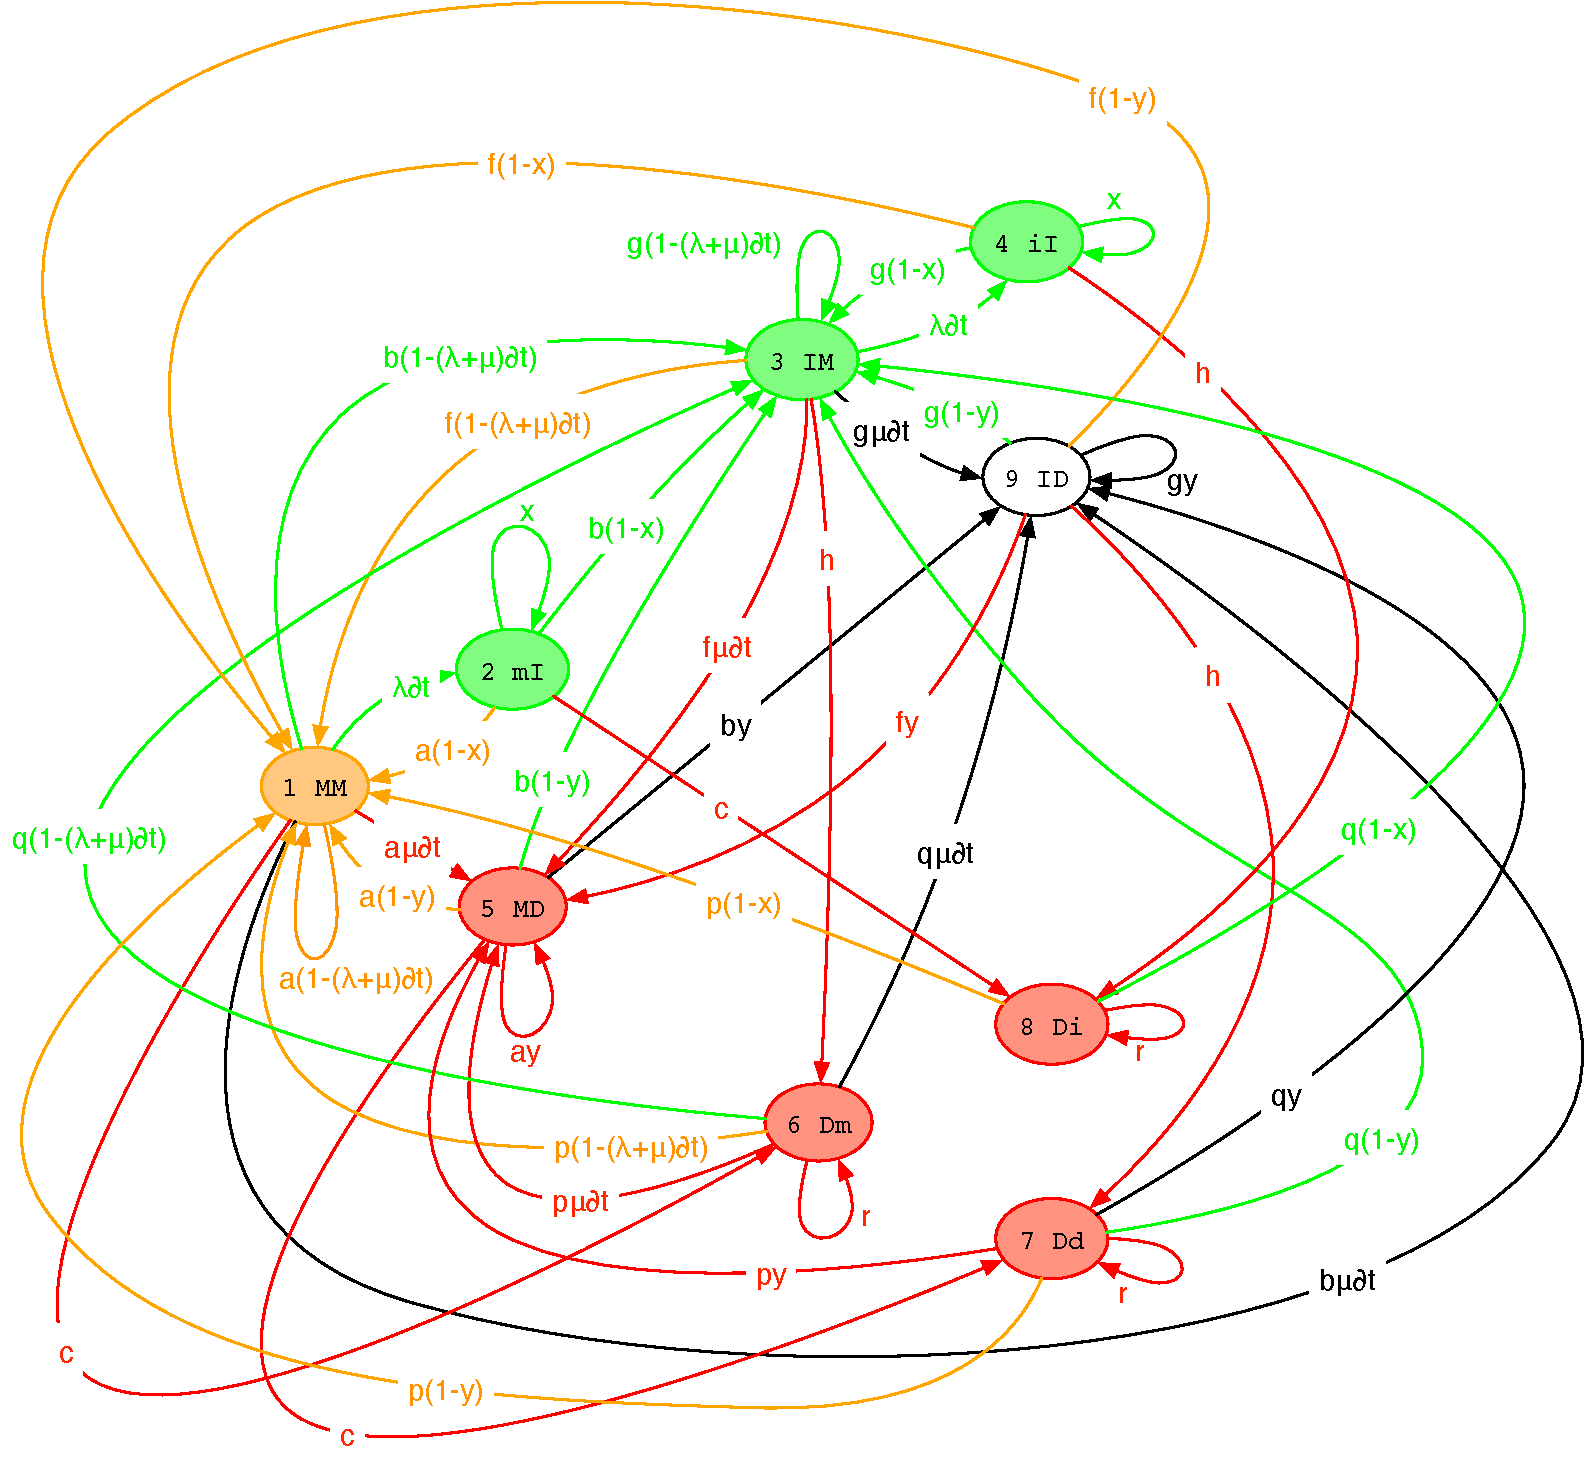
\includegraphics[width=\textwidth]{PairInstant.pdf}

\[
 {\bf U} =
  \begin{pmatrix}
a (1-(\lambda+\mu) \delta_t) & \lambda \delta_t & b (1-(\lambda+\mu) \delta_t) & 0 & a \mu \delta_t & c & 0 & 0 & b \mu \delta_t \\
a (1-x) & x & b (1-x) & 0 & 0 & 0 & 0 & c & 0 \\
f (1-(\lambda+\mu) \delta_t) & 0 & g (1-(\lambda+\mu) \delta_t) & \lambda \delta_t & f \mu \delta_t & h & 0 & 0 & g \mu \delta_t \\
f (1-x) & 0 & g (1-x) & x & 0 & 0 & 0 & h & 0 \\
a (1-y) & 0 & b (1-y) & 0 & a y & 0 & c & 0 & b y \\
p (1-(\lambda+\mu) \delta_t) & 0 & q (1-(\lambda+\mu) \delta_t) & 0 & p \mu \delta_t & r & 0 & 0 & q \mu \delta_t \\
p (1-y) & 0 & q (1-y) & 0 & p y & 0 & r & 0 & q y \\
p (1-x) & 0 & q (1-x) & 0 & 0 & 0 & 0 & r & 0 \\
f (1-y) & 0 & g (1-y) & 0 & f y & 0 & h & 0 & g y    
  \end{pmatrix}
\]

State sets are
$\sigma_M=\{1\}$ (orange),
$\sigma_I=\{2,3,4\}$ (green),
$\sigma_D=\{5,6,7,8\}$ (red),
$\sigma_N=\{9\}$ (white).
  
\subsection{Algebraic ODEs for $T_{XY}$ under GGI model}

Derived in \cite{Holmes2020}.

\begin{eqnarray*}
S_I(t) & = & \exp\left(\frac{\lambda t}{1-x}\right)-1 \\
S_D(t) & = & \exp\left(\frac{\mu t}{1-y}\right)-1 \\
 T_{ij}(0) & = & \mbox{1 if $i=j=M$, 0 otherwise}
\\
  \frac{d}{dt} T_{MM}(t) & = &
  \mu \frac{b f (1-y)}{1 - g y}-(\lambda +\mu )a
  \nonumber \\
  \frac{d}{dt} T_{MI}(t) & = &
  -\mu \frac{b (1-g)}{1 - g y} + \lambda (1-b)
  \nonumber \\
  \frac{d}{dt} T_{IM}(t) & = &
  \lambda a - \mu \frac{f (1-g) (b (1-r)+c q)}{(1 - g y) (f (1-r)+h p)}
  \nonumber \\
  \frac{d}{dt} T_{DI}(t) & = &
  \mu \frac{(1-g) (b (1-r-h q)+c g q)}{(1-g y) (f (1-r)+h p)}
\end{eqnarray*}

with $T_{MM}(0)=1$ and $T_{MI}(0)=T_{IM}(0)=T_{DI}(0)=0$.

The substitution matrix $E_M(x,y)$ for the match state is
the matrix exponential $\exp({\bf Q}t)_{xy}$, for which a Pad\'{e} approximant
or other power series expansion can be used in order to remain automatically differentiable under frameworks like PyTorch or Jax. % \cite{MolerVanLoan2003}
For the insert states the emission weights are $E_I(\epsilon,y)=\pi_y$,
and for the delete states $E_D(x,\epsilon)=1$.

\subsubsection{A simpler form for the GGI ODEs}

Rewrite the GGI ODEs with $a \equiv T_{MM}, b \equiv T_{MI}, u \equiv T_{IM}, v \equiv T_{DI}, S \equiv S_I$:
\begin{eqnarray*}
  \frac{da}{dt} & = & \frac{\mu (1-y) b u}{S - y(S-b-v)} - (\lambda +\mu ) a \\
  \frac{db}{dt} & = & -\frac{\mu (b+v) b}{S - y(S-b-v)} + \lambda (1-b) \\
  \frac{du}{dt} & = & -\frac{\mu (b+v) u}{S - y(S-b-v)} + \lambda a \\
  \frac{dv}{dt} & = & \frac{\mu (b+v) (S-v)}{S - y(S-b-v)} \\
  S & = & \exp\left(\frac{\lambda t}{1-x}\right)-1
\end{eqnarray*}
with $a(0)=1$, $b(0)=u(0)=v(0)=0$,
$a'(0)=-\lambda-\mu$, $b'(0)=u'(0)=\lambda$, and $v'(0)=0$.

Note that the denominator vanishes at $t=0$, so these formulae are undefined there.
However, in the limit $t \to 0$, the counts are obtainable to first order in $t$ by inspection of $\mathbb{G}(\delta t)$,
%\begin{eqnarray*}
%  a(\delta t) & = & 1 - (\lambda+\mu) \delta t + o(\delta t) \\
%  b(\delta t) & = & \lambda \delta t + o(\delta t) \\
%  u(\delta t) & = & \lambda \delta t + o(\delta t) \\
%  v(\delta t) & = & o(\delta t) \\
%  S(\delta t) & = & \frac{\lambda}{1-x} \delta t + o(\delta t)
%\end{eqnarray*}
yielding the expressions for the derivatives at the boundary.
It is straightforward to use L'H\^{o}pital's rule to verify that these first-order approximations satisfy the ODEs as $t \to 0$.
%First we need to rewrite all the ODEs as rational functions
%\begin{eqnarray*}
%  \frac{da}{dt} & = & \frac{\mu (y-1) b u - (\lambda +\mu ) a \left( y(S-b-v) - S \right)}{y(S-b-v) - S} \\
%  \frac{db}{dt} & = & \frac{\mu (b+v) b + \lambda (1-b) \left( y(S-b-v) - S \right)}{y(S-b-v) - S} \\
%  \frac{du}{dt} & = & \frac{\mu (b+v) u + \lambda a \left( y(S-b-v) - S \right)}{y(S-b-v) - S} \\
%  \frac{dv}{dt} & = & \frac{\mu (b+v) (v-S)}{y(S-b-v) - S}
%\end{eqnarray*}
%Then use $\lim_{t\to0} f(t)/g(t) = f'(0)/g'(0)$:
%\begin{eqnarray*}
%  a'(0) & = & \frac{\mu (y-1) (b' u + u' b) - (\lambda +\mu ) \left( a' \left( y(S-b-v) - S \right) + a \left( y(S'-b'-v') - S' \right) \right)}{y(S'-b'-v') - S'} \\
%  b'(0) & = & \frac{\mu \left((b'+v') b + (b+v) b' \right) + \lambda \left( -b' \left( y(S-b-v) - S \right) + (1-b) \left( y(S'-b'-v') - S' \right) \right)}{y(S'-b'-v') - S'} \\
%  u'(0) & = & \frac{\mu \left((b'+v') u + (b+v) u' \right) + \lambda \left( a' \left( y(S-b-v) - S \right) + a \left( y(S'-b'-v') - S' \right) \right)}{y(S'-b'-v') - S'} \\
%  v'(0) & = & \frac{\mu \left( (b'+v') (v-S) + (b+v) (v'-S') \right)}{y'(S'-b'-v') - S'}
%\end{eqnarray*}
%
% etc.

% Observation: note that $S-b-v=G$ (in the denominator). Note also that $b+v=S-G$. Maybe $G$ is a better choice of variable than $u$? What is the ODE for $G$?
% (Answer: it does not seem to be possible to express $G'$ in a form that does not depend on $b$, so it is presumably no easier to solve than $u$.)

The variables $(a,b,u,v)$ represent expected counts and are nonnegative always.
Further, for $t>0$ (and assuming $\lambda,\mu > 0$), we know that
$a < \exp(-\mu t)$, $a+b<1$, $a+u<1$, $b+v<S$, and $v<D-(1-a-u)$
where $D \equiv S_D = \exp\left(\frac{\mu t}{1-y}\right) - 1$.

As $t \to \infty$ we have $S \simeq \exp\left(\frac{\lambda t}{1-x}\right)$ and (because ancestral residues are inevitably deleted) $a \to 0$.
\textcolor{red}{What else can we say about the asymptotic behavior of these counts as time gets large?
(This could be useful in modeling them numerically, if we can't find algebraic solutions to the ODEs.)}

A problem with numerically integrating these ODEs is that $S$, $D$, and $v$ get very large and overflow.
We can stabilize them by transforming to variables $(a,b,u,q,L,M)$ where $L=1/(S+1)$, $M=1/(D+1)$, $q=v/D$, and $q'=(v/D)'=(v'-qD')/D$.
Then

% We could obtain ODEs directly for the probabilities $a,b,f,q$
% by using $f'=(u/S)'=(u'-fS')/S$, $q'=(v/D)'=(v'-qD')/D$
% and making the above substitutions to express $(a,b,u,v)$ in terms of $(a,b,f,q,S,D)$
% \begin{eqnarray*}
%   \frac{da}{dt} & = & \frac{\mu (1-y) b f S}{S - y(S-b-q D)} - (\lambda +\mu ) a \\
%   \frac{db}{dt} & = & -\frac{\mu (b+q D) b}{S - y(S-b-q D)} + \lambda (1-b) \\
%   \frac{df}{dt} & = & \frac{1}{S} \left( -\frac{\mu (b+q D) f S}{S - y(S-b-q D)} + \lambda a - \frac{f \lambda(S+1)}{1-x} \right) \\
%   \frac{dq}{dt} & = & \frac{1}{D} \left( \frac{\mu (b+q D) (S-q D)}{S - y(S-b-q D)} - \frac{q \lambda(D+1)}{1-y} \right) \\
%   S & = & \exp\left(\frac{\lambda t}{1-x}\right)-1 \\
%   D & = & \exp\left(\frac{\mu t}{1-y}\right)-1
% \end{eqnarray*}
% with $a(0)=1$, $b(0)=q(0)=0$, $f(0)=1-x$,
% $a'(0)=-\lambda-\mu$, $b'(0)=\lambda$, $f'(0)=1-x$, and $q'(0)=0$.   % That f'(0)=1-x is weird but apparently correct.
% 
% These probability ODEs might be expected to be more stable than the ODEs for the counts (since $(a,b,f,q)$ are all between 0 and 1).
% Maybe it would be simpler to work with $(a,b,u,q)$ since it's really only $v$ that explodes (the others are all bounded by $[0,1]$ already, and $f'$ is more complicated than $u'$).
% Then we should multiply numerators and denominators by $1/S$ and/or $1/D$ for stability,
% or even set $L=1/(S+1)$ and $M=1/(D+1)$ and use those instead of $S$ and $D$.
% 
% Thus
% \begin{eqnarray*}
%   \frac{da}{dt} & = & \frac{\mu (1-y) b u}{S - y(S-b-q D)} - (\lambda +\mu ) a \\
%   \frac{db}{dt} & = & -\frac{\mu (b+q D) b}{S - y(S-b-q D)} + \lambda (1-b) \\
%   \frac{du}{dt} & = & -\frac{\mu (b+q D) u}{S - y(S-b-q D)} + \lambda a \\
%   \frac{dq}{dt} & = & \frac{1}{D} \left( \frac{\mu (b+q D) (S-q D)}{S - y(S-b-q D)} - \frac{q \lambda(D+1)}{1-y} \right) \\
%   S & = & \exp\left(\frac{\lambda t}{1-x}\right)-1 \\
%   D & = & \exp\left(\frac{\mu t}{1-y}\right)-1
% \end{eqnarray*}
% 
% Or

\begin{eqnarray*}
  \frac{da}{dt} & = & \frac{\mu (1-y) b u L M}{M (1 - y) + L q y + L M (y (1 + b - q) - 1)} - (\lambda +\mu ) a \\
  \frac{db}{dt} & = & -\frac{\mu (bM+q(1-M)) b L}{M (1 - y) + L q y + L M (y (1 + b - q) - 1)} + \lambda (1-b) \\
  \frac{du}{dt} & = & -\frac{\mu (bM+q(1-M)) u L}{M (1 - y) + L q y + L M (y (1 + b - q) - 1)} + \lambda a \\
  \frac{dq}{dt} & = & \frac{1}{1-M} \left( \frac{\mu (bM+q(1-M)) (M(1-L)-qL(1-M))}{M (1 - y) + L q y + L M (y (1 + b - q) - 1)} - \frac{q \lambda}{1-y} \right) \\
  L & = & \exp\left(-\frac{\lambda t}{1-x}\right) \\
  M & = & \exp\left(-\frac{\mu t}{1-y}\right)
\end{eqnarray*}
with $a(0)=1$, $b(0)=u(0)=q(0)=0$,
$a'(0)=-\lambda-\mu$, $b'(0)=u'(0)=\lambda$, and $q'(0)=0$.

\textcolor{red}{There may be a lesson here for the general case: it is more stable to solve numerically in probability space, not count space.}

Note the relationship between the variables in these ODEs and the transition probabilities of $\mathbb{F}(t)$:
\begin{eqnarray*}
\begin{pmatrix}
a & b & c \\
f & g & h \\
p & q & r 
\end{pmatrix}
& = &
\begin{pmatrix}
a & b & 1-a-b \\
u/S & (S-b-v)/S & (b+v-u)/S \\
(1-a-u)/D & v/D & (D+a+u-v-1)/D 
\end{pmatrix}
\\
& = &
\begin{pmatrix}
a & b & 1-a-b \\
\frac{L}{1-L} u & 1 - \frac{L}{1-L} \left( b + \frac{1-M}{M} q \right) & \frac{L}{1-L} (b + \frac{1-M}{M} q - u) \\
\frac{M}{1-M} (1 - a - u) & q & 1 - q -  \frac{M}{1-M} \left( 1 - a - u \right)
\end{pmatrix}
\end{eqnarray*}

Conversely, $u=fS$ and $v=qD$, which gives closed-form solutions in the special case of TKF91 (see below).



\subsection{TKF91 as exactly-solved special case of GGI model}

When $x=y=0$ the model is TKF91 \cite{ThorneEtAl91}
with solution
$
\begin{pmatrix}
a & b & c \\
f & g & h \\
p & q & r 
\end{pmatrix}
=
\begin{pmatrix}
(1-\beta)\alpha & \beta & (1-\beta)(1-\alpha) \\
(1-\beta)\alpha & \beta & (1-\beta)(1-\alpha) \\
(1-\gamma)\alpha & \gamma & (1-\gamma)(1-\alpha)
\end{pmatrix}
$
where
$\alpha = \exp(-\mu t)$,
$\beta = \frac{\lambda \left( \exp(-\lambda t) - \exp(-\mu t) \right)}{\mu \exp(-\lambda t) - \lambda \exp(-\mu t)}$
and
$\gamma = 1 - \frac{\mu \beta}{\lambda (1 - \alpha)}$.

In terms of our ODE variables $(a,b,u,v)$
\begin{eqnarray*}
  a & = & \frac{\mu - \lambda}{\mu L - \lambda M} LM \\
  b & = & \frac{\lambda}{\mu L - \lambda M} (L - M) \\
  u & = & \frac{\mu - \lambda}{\mu L - \lambda M} M(1-L) \\
  v & = & \frac{\mu - \lambda}{\mu L - \lambda M} - 1
\end{eqnarray*}
with $L=\exp(-\lambda t)$ and $M=\exp(-\mu t)$.
\textcolor{red}{This does suggest trial solutions, including perhaps a simpler form for the $(b,v)$ subsystem.}


\subsection{GGI model transition likelihood}

The following recipe refers to the case where the alignment is specified.
If it's unspecified, use the Forward algorithm to sum over alignments.

The pairwise alignment of ancestor $i$ and descendant $j$ can be summarized by two lists:
\begin{itemize}
    \item The list $A_M$ of pairs of aligned characters $(\omega,\omega')$ from ancestor ${\cal S}(0)$ and descendant ${\cal S}(t)$;
    \item The list $A_{ID}$ of pairs of unaligned gap sequences $(\delta,\delta')$ that were deleted and inserted in between.
\end{itemize}

The alignment probability, computable in time $O(L)$ (and in practice very fast), is
\[
P(A_M,A_{ID},{\cal S}(t)|{\cal S}(0)) =
\prod_{(\omega,\omega') \in A_M} \exp({\bf Q}t)_{\omega \omega'}
\prod_{(\delta,\delta') \in A_{ID}} G(|\delta|,|\delta'|,t)
\prod_{\omega'\in \delta'} \pi_{\omega'}
\]

where $G(i,j,t)$ is the probability that between the next pair of aligned characters in ${\cal S}(0)$ and ${\cal S}(t)$,
there were $i$ characters deleted from ${\cal S}(0)$ 
and $j$ characters inserted into ${\cal S}(t)$,
with no homology
\begin{eqnarray*}
G(i,j,t) & = &
\left\{ \begin{array}{ll}
a & i=j=0 \\
cr^{i-1}p & i>0, j=0 \\
bg^{j-1}f & i=0, j>0 \\
\displaystyle
g^{j-1} r^{i-1}
\left(
bhp + cqf +
\sum_{k=1}^{\min(i,j)} C(i,j,k,t)
\right)
& i>0, j>0
\end{array} \right.
\\
C(i,j,k,t) & = &
\left( \frac{hq}{gr} \right)^k
\binom{i-1}{k-1} \binom{j-1}{k-1} \frac{1}{k^2}
\left( b(j-k)(rfk + hp(i-k)) + c(i-k)(gpk + qf(j-k)) \right)
\end{eqnarray*}

% The unobserved index $k$ counts "unnecessary" zig-zags on the Pair HMM state path
% ($D \to I \to D$ or $I \to D \to I$).

% With i D's, and j I's,
% and an initial transition M->I (b) and return I->M (f),
% you can have at most min(i,j-1) zigzags
% There are (j-1 choose k) ways of picking the k I's before which each crossover takes place
% There are (i-1 choose k-1) ways of picking the k-1 D's before which each return (except the last one) takes place
% 
% With i D's, and j I's,
% and an initial transition M->I (b) and return D->M (p),
% you can have at most min(i-1,j-1) zigzags
% There are (j-1 choose k) ways of picking the k I's before which each crossover takes place
% There are (i-1 choose k) ways of picking the k D's before which each return takes place
% 
% With i D's, and j I's,
% and an initial transition M->D (c) and return I->M (f),
% you can have at most min(i-1,j-1) zigzags
% There are (i-1 choose k) ways of picking the k D's before which each crossover takes place
% There are (j-1 choose k) ways of picking the k I's before which each return takes place
% 
% With i D's, and j I's,
% and an initial transition M->D (c) and return D->M (p),
% you can have at most min(i-1,j) zigzags
% There are (i-1 choose k) ways of picking the k D's before which each crossover takes place
% There are (j-1 choose k-1) ways of picking the k-1 I's before which each return (except the last one) takes place


\subsection{Phylogenetic alignment under GGI model}

Both forms of the pairwise likelihood (alignment specified, or unspecified) can be extended to multiple sequences on a phylogeny.
Upgrade $\exp({\bf Q}t)$ to Felsenstein pruning. % \cite{Felsenstein81}.

For the alignment-unspecified form, use transducer composition to obtain $N$-sequence HMMs \cite{SilvestreRyanEtAl2020}.
The resulting Forward algorithm is $O(L^N)$.
To ameliorate this, discard all but a few representative sample paths \cite{WestessonEtAl2012},
or use MCMC \cite{RedelingsSuchard2007}.

\bibliographystyle{unsrt}
\bibliography{references}


\end{document}
